\documentclass{article}

\usepackage{siunitx}
\usepackage{tikz} % To generate the plot from csv
\usepackage{pgfplots}

\pgfplotsset{compat=newest} % Allows to place the legend below plot
\usepgfplotslibrary{units} % Allows to enter the units nicely

\sisetup{
    round-mode          = places,
    round-precision     = 2,
}

\begin{document}

    \begin{figure}[h!]
        \begin{center}
            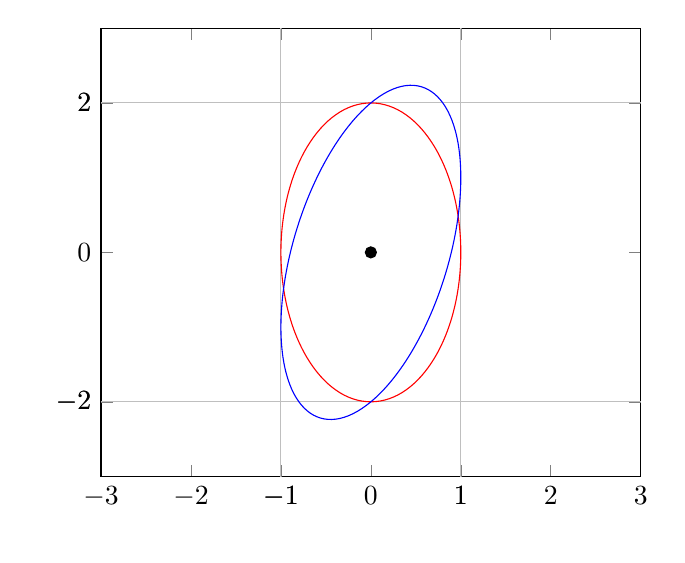
\begin{tikzpicture}
                \begin{axis}[
                    xmin=-3,   xmax=3,
                    ymin=-3,   ymax=3,
                    extra x ticks={-1,1},
                    extra y ticks={-2,2},
                    extra tick style={grid=major},
                ]
                    \draw[red] \pgfextra{
                        \pgfpathellipse{\pgfplotspointaxisxy{0}{0}}
                        {\pgfplotspointaxisdirectionxy{1}{0}}
                        {\pgfplotspointaxisdirectionxy{0}{2}}
                        % see also the documentation of
                        % 'axis direction cs' which
                        % allows a simpler way to draw this ellipse
                        };
                    \draw[blue] \pgfextra{
                        \pgfpathellipse{\pgfplotspointaxisxy{0}{0}}
                        {\pgfplotspointaxisdirectionxy{1}{1}}
                        {\pgfplotspointaxisdirectionxy{0}{2}}
                    };
                    \addplot [only marks,mark=*] coordinates { (0,0) };
                \end{axis}
            \end{tikzpicture}
            \caption{My first autogenerated plot.}
        \end{center}
    \end{figure}

\end{document}